\documentclass{beamer}
%
% Choose how your presentation looks.
%
% For more themes, color themes and font themes, see:
% http://deic.uab.es/~iblanes/beamer_gallery/index_by_theme.html
%
\mode<presentation>
{
  \usetheme{default}      % or try Darmstadt, Madrid, Warsaw, ...
  \usecolortheme{default} % or try albatross, beaver, crane, ...
  \usefonttheme{default}  % or try serif, structurebold, ...
  \setbeamertemplate{navigation symbols}{}
  \setbeamertemplate{caption}[numbered]
  \setbeamertemplate{footline}[frame number]
} 

\usepackage[english]{babel}
\usepackage[utf8x]{inputenc}
\usepackage{listings}
\usepackage{courier}

\title[2016-03-14-scaroot]{Accessing ROOT and C++ functions in Spark}
\author{Jim Pivarski}
\institute{Princeton University --- DIANA}
\date{March 14, 2016}

\xdefinecolor{darkblue}{rgb}{0.1,0.1,0.7}
\definecolor{mygreen}{rgb}{0,0.6,0}
\definecolor{mygray}{rgb}{0.5,0.5,0.5}
\definecolor{mymauve}{rgb}{0.58,0,0.82}

\lstset{ %
  backgroundcolor=\color{white},   % choose the background color
  basicstyle=\ttfamily\scriptsize,        % size of fonts used for the code
  breaklines=true,                 % automatic line breaking only at whitespace
  captionpos=b,                    % sets the caption-position to bottom
  commentstyle=\color{mygreen},    % comment style
  escapeinside={\%*}{*)},          % if you want to add LaTeX within your code
  keywordstyle=\color{blue},       % keyword style
  stringstyle=\color{mymauve},     % string literal style
  showstringspaces=false
}

\lstdefinelanguage{scala}{
  morekeywords={abstract,case,catch,class,def,%
    do,else,extends,false,final,finally,%
    for,if,implicit,import,match,mixin,%
    new,null,object,override,package,%
    private,protected,requires,return,sealed,%
    super,this,throw,trait,true,try,%
    type,val,var,while,with,yield},
  otherkeywords={=>,<-,<\%,<:,>:,\#,@},
  sensitive=true,
  morecomment=[l]{//},
  morecomment=[n]{/*}{*/},
  morestring=[b]",
  morestring=[b]',
  morestring=[b]"""
}

\begin{document}

\begin{frame}
  \titlepage
\end{frame}

% Uncomment these lines for an automatically generated outline.
%\begin{frame}{Outline}
%  \tableofcontents
%\end{frame}

\begin{frame}{}
My work on integrating ROOT and Spark has split into:
\begin{description}
\item[ScaROOT:] Call ROOT functions (and arbitrary C++) from Scala, and therefore Spark, Hadoop, etc.
\item[root2avro:] Bulk data flow from ROOT files to other file formats or streaming into Spark, Hadoop, etc.
\end{description}

\vfill
For the last few weeks, \textcolor{darkblue}{root2avro} has been my main focus, but I recently got \textcolor{darkblue}{ScaROOT} into usable shape.

\vfill
\textcolor{darkblue}{root2avro} isn't a special case of \textcolor{darkblue}{ScaROOT} for reasons you'll see in a moment.
\end{frame}

\begin{frame}{}
Documented with unit tests and examples on the GitHub wiki page (\url{https://github.com/diana-hep/scaroot}).

\vspace{0.5 cm}
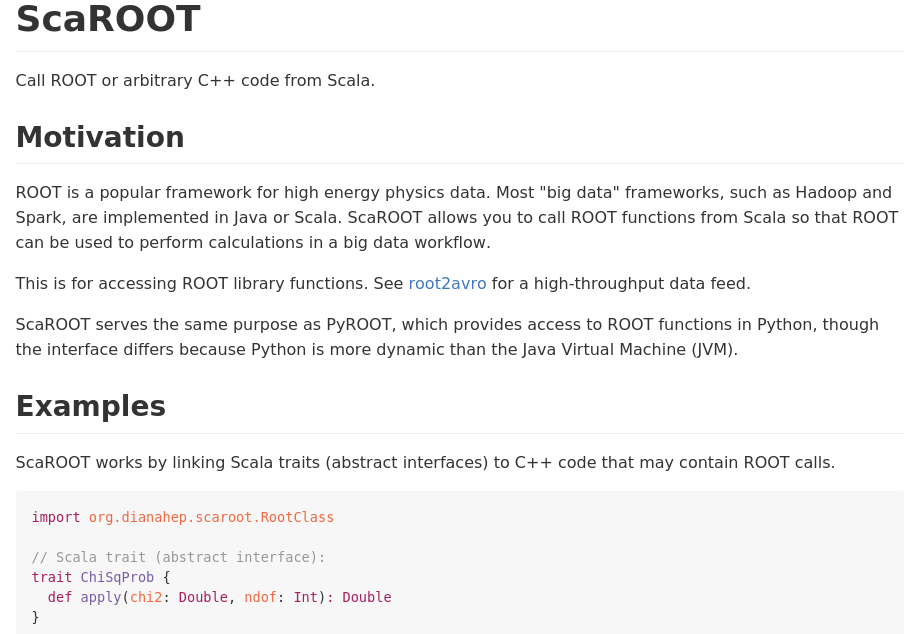
\includegraphics[width=\linewidth]{wiki.png}
\end{frame}

\begin{frame}{Interface}

\begin{block}{}
\vspace{-\baselineskip}
PyROOT dynamically makes proxies to ROOT functions when they're called, so that working in Python is approximately the same as working in CINT/Cling (replacing ``{\tt ->}'' and ``{\tt ::}'' with ``{\tt .}'').
\end{block}

\vfill
\begin{uncoverenv}<2->
\begin{block}{}
\vspace{-\baselineskip}
Scala (and Java) are compiled languages, so field names of classes have to be declared in advance. Classes can be defined on the fly (in a private ClassLoader), but the main program can only use them if they adhere to a predefined interface (abstract class).
\end{block}
\end{uncoverenv}

\vfill
\begin{uncoverenv}<3->
\begin{block}{}
\vspace{-\baselineskip}
We therefore ask the user to define a Scala interface that is satisfied by a C++ class. The C++ class can use any ROOT functions.
\end{block}
\end{uncoverenv}
\end{frame}

\begin{frame}[fragile]{Example}
\begin{lstlisting}[language=scala]
import org.dianahep.scaroot.RootClass

// Scala trait (abstract class with virtual methods):
trait ChiSqProb {
  def apply(chi2: Double, ndof: Int): Double
}

// C++ class definition that satisfies the interface:
val chiSqProbClass = RootClass[ChiSqProb]("""
class ChiSqProb {
public:
  double apply(double chi2, int ndof) {
    return ROOT::Math::chisquared_cdf(chi2, ndof);
  }
};
""")

// Create an instance:
val chiSqProb = chiSqProbClass.newInstance

// And use it:
chiSqProb.apply(53.8, 50)   // or just chiSqProb(53.8, 50)
                            // because 'apply' is 'operator()'
0.6689797343068249
\end{lstlisting}
\end{frame}

\begin{frame}{How it works}
\begin{itemize}
\item The use of ``{\tt RootClass[ChiSqProb]}'' in the code invokes a compile-time macro that generates custom hooks for the ``{\tt ChiSqProb}'' trait.
\item These hooks connect to ROOT through JNA (same process, no serialization, just a memory-to-memory copy).
\item ROOT's {\tt TInterpreter} is invoked to compile the code and give the JVM a direct pointer to the class.
\item At execution time, the method arguments are copied from Java's memory heap to C++'s, the function is called, and the return values are copied back, all within a single process.
\end{itemize}

\vfill
\hspace{-0.83 cm} \textcolor{darkblue}{\Large Who would use it}
\begin{itemize}
\item Users doing high-throughput calculations (e.g.\ skimming) on Spark: the round-trip time between Spark and ROOT is minimized.
\item Or a library of predefined interfaces provided to the user.
\end{itemize}
\end{frame}

\begin{frame}{Capabilities}
\begin{itemize}
\item The C++ code is not fixed until it is used to create an object. It could be dynamically generated for ``just in time'' flexibility and efficiency.
\item {\tt RootClass} objects are serializable (as the C++ string!) so that they can be passed to a remote Spark workflow.
\end{itemize}

\vfill
\hspace{-0.83 cm} \textcolor{darkblue}{\Large Limitations}

\begin{itemize}
\item The class must have a zero-argument constructor.
\item Parameter types and return types must be primitives (numbers, strings, or an opaque {\tt com.sun.jna.Pointer} to C++ data).
\item (The appropriate version of) ROOT needs to be installed across the Spark cluster, accessible via {\tt LD\_LIBRARY\_PATH} like any other natively compiled program.
\end{itemize}
\end{frame}

\begin{frame}{Status}
\begin{itemize}
\item Works, but has {\it no error checking.} Any mistake causes segmentation fault (will fix).
\item Has not been tested in Spark yet. (Does anyone have an application they're eager to try? Want to work with me?)
\end{itemize}

\vfill
\vfill
\hspace{-0.83 cm} \textcolor{darkblue}{\Large Possible extensions}
\begin{itemize}
\item Could build a library of common functions (histograms and such) by hand.
\item Could exhaustively search the space of ROOT functions by a graph traversal on {\tt TInterpreter}. This would be a better analogy with PyROOT, but statically compiled.
\end{itemize}

\vfill
\vfill
\hspace{-0.83 cm} \textcolor{darkblue}{\Large Why is this not a data feed (root2avro)?}
\begin{itemize}
\item With a primitives-only interface, each complex data structure (CMSSW, ART, Bacon, \ldots) would have to be adapted by hand. We want to recognize these structures automatically.
\end{itemize}
\end{frame}

\begin{frame}{Status of root2avro}
\begin{itemize}
\item All known data types that can be found in TTrees are handled, with a framework that can easily add new ones as they're discovered.
\item Successfully examined and converted a Bacon-tuple to JSON.
\item All JSON-writing functions have been supplanted with Avro-writing functions.
\end{itemize}

\vfill
\vfill
\hspace{-0.83 cm} \textcolor{darkblue}{\Large What's next?}
\begin{enumerate}
\item Convert Matteo and Christina's Bacon-tuples to Avro files, load into a Spark cluster.
\item Fix any bugs and segmentation faults along the way.
\item Stream ROOT data into Scala using two processes (Avro data pipe).
\item Wrap this up in a Spark InputRDD and/or DataFrame (they're different).
\item Stream ROOT data into Scala directly into the JVM, still using Avro as the common language.
\end{enumerate}
\end{frame}

\begin{frame}[fragile]{Example Avro schema from a Bacon-tuple}
\tiny
\begin{verbatim}
{"type": "record",
 "name": "Events",
 "fields": [
   {"name": "GenParticle", "type": {"type": "array", "items": {"type": "record",
    "name": "baconhep::TGenParticle",
    "fields": [
      {"name": "parent", "type": "int"},
      {"name": "pdgId", "type": "int"},
      {"name": "status", "type": "int"},
      {"name": "pt", "type": "float"},
      {"name": "eta", "type": "float"},
      {"name": "phi", "type": "float"},
      {"name": "mass", "type": "float"},
      {"name": "y", "type": "float"}
    ]
   }}},
   {"name": "LHEWeight", "type": {"type": "array", "items": {"type": "record",
    "name": "baconhep::TLHEWeight",
    "fields": [
      {"name": "id", "type": "int", "doc": "parton flavor PDG ID"},
      {"name": "weight", "type": "float", "doc": "generator-level event weight"}
    ]
   }}},
   {"name": "Electron", "type": {"type": "array", "items": {"type": "record",
    "name": "baconhep::TElectron",
    "fields": [
      {"name": "pt", "type": "float", "doc": "kinematics"},
      {"name": "eta", "type": "float", "doc": "kinematics"},
      {"name": "phi", "type": "float", "doc": "kinematics"},
      {"name": "scEt", "type": "float", "doc": "supercluster kinematics"},
      {"name": "scEta", "type": "float", "doc": "supercluster kinematics"},
      {"name": "scPhi", "type": "float", "doc": "supercluster kinematics"},
      {"name": "ecalEnergy", "type": "float", "doc": "ECAL energy"},
    ...
\end{verbatim}
\end{frame}

\end{document}
